\section{Flywheel study}

\subsection{System of differential equations}
As described in figure \ref{fig:Flywheel force diagram} we will use two variables to describe the flywheel position: $r$, $\theta$ 
We will use the change of variables $\alpha =\pi/2 - \theta$

Using equation \ref{flywheel equation}:
\[\tau_{flywheel} = \ddot{\theta}*I_{flywheel}(r) + m_{cylinder} * g * (r - r_{max}) * \sin{\theta}\]
\begin{figure}[ht]
	\centering
	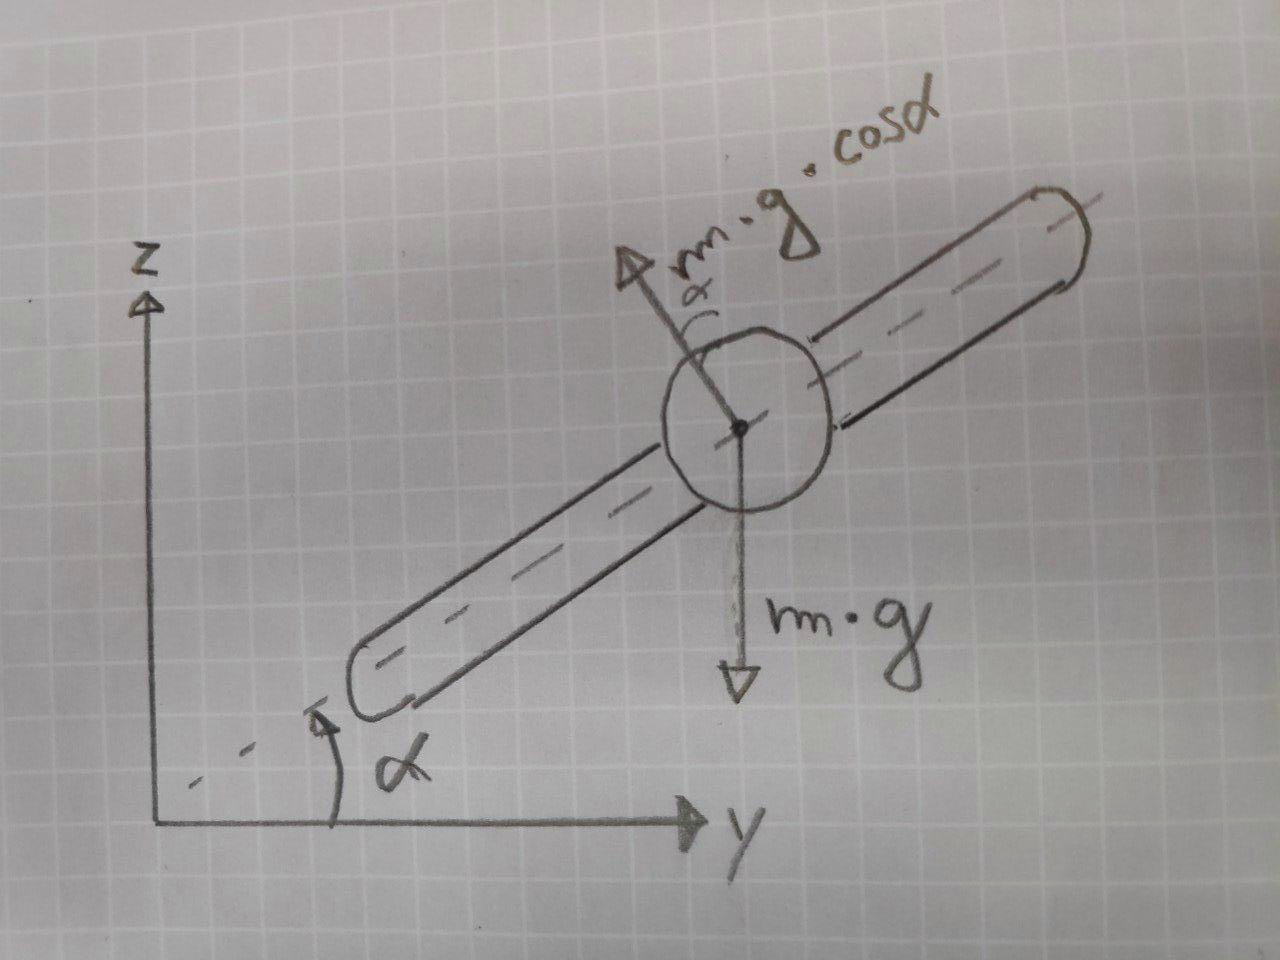
\includegraphics[width=10cm]{img/cylinder_forces.png}
	\caption{Cylinder force diagram}
	\label{fig:Cylinder force diagram}
\end{figure}

As seen in figure \ref{fig:Cylinder force diagram}, we can deduce newtons equation for the distance from the cylinder to the center $r$. Note that we are adding the centrifugal force term due to the non-inertial frame.
\[\ddot{r} * m = -m * g * sin(\pi/2-\theta) + m * r * \dot{\theta}^2 \]
\[\ddot{r} = -g * sin(\pi/2-\theta) + r * \dot{\theta}^2 \]

The variables we will be using for our ODE system are: $r$,$\dot{r}$,$\theta$,$\dot{\theta}$


\[
\begin{cases}
    \dot{r} = \dot{r}\\
    \ddot{r} = -g * sin(\pi/2-\theta) + r * \dot{\theta}^2\\
    \dot{\theta} = \dot{\theta}\\
    \ddot{\theta} = \frac{\tau_{flywheel}-m_{cylinder} * g * (r - r_{max}) * \sin{\theta}}{I_{flywheel}(r)} \\    
\end{cases}
\]

Our initial conditions will be the the free cylinder lying on the bottom of the flywheel and the flywheel turning at a speed $\theta_0$:
\[
    \begin{cases}
        r = r_{max} \\
        \dot{r} = 0\\
        \theta = \pi\\
        \dot{\theta} = \theta_0\\
    \end{cases}
\]

We will use a poincare map to simulate the bounce with the end of the guides at $r=r_{min}$ and $r=r_{max}$. At each bounce we will reduce its kinetic energy by a percentage $bounce\_percentage$  


